% ============================================================
% FIG 7 — Per-Layer Latency Breakdown
% Horizontal stacked bar using real per-stage mean latency
% from Fig 11 (120-scenario diagnostic harness, log scale in paper).
% Values read from the paper's Fig 11 (approximate, log scale):
%   PKI:        ~0.5 ms
%   B1 (SCSV):  ~1.5 ms
%   MBD:        ~3.0 ms
%   B2 (CSIA):  ~8.0 ms
%   CP:         ~0.8 ms
%   Synthesizer:~18.0 ms
%   B3 (bridge):~71.0 ms   (dominant stage)
%   Fusion:     ~4.0 ms
% Total ~106.8 ms (consistent with reported mean 110 ms)
% ============================================================
% PREAMBLE:
%   \usepackage{tikz}
%   \usepackage{xcolor}
%   \usetikzlibrary{arrows.meta, positioning, calc}
%
% PLACEMENT: single column
%   \begin{figure}[t]
%     \centering
%     % ============================================================
% FIG 7 — Per-Layer Latency Breakdown
% Horizontal stacked bar using real per-stage mean latency
% from Fig 11 (120-scenario diagnostic harness, log scale in paper).
% Values read from the paper's Fig 11 (approximate, log scale):
%   PKI:        ~0.5 ms
%   B1 (SCSV):  ~1.5 ms
%   MBD:        ~3.0 ms
%   B2 (CSIA):  ~8.0 ms
%   CP:         ~0.8 ms
%   Synthesizer:~18.0 ms
%   B3 (bridge):~71.0 ms   (dominant stage)
%   Fusion:     ~4.0 ms
% Total ~106.8 ms (consistent with reported mean 110 ms)
% ============================================================
% PREAMBLE:
%   \usepackage{tikz}
%   \usepackage{xcolor}
%   \usetikzlibrary{arrows.meta, positioning, calc}
%
% PLACEMENT: single column
%   \begin{figure}[t]
%     \centering
%     % ============================================================
% FIG 7 — Per-Layer Latency Breakdown
% Horizontal stacked bar using real per-stage mean latency
% from Fig 11 (120-scenario diagnostic harness, log scale in paper).
% Values read from the paper's Fig 11 (approximate, log scale):
%   PKI:        ~0.5 ms
%   B1 (SCSV):  ~1.5 ms
%   MBD:        ~3.0 ms
%   B2 (CSIA):  ~8.0 ms
%   CP:         ~0.8 ms
%   Synthesizer:~18.0 ms
%   B3 (bridge):~71.0 ms   (dominant stage)
%   Fusion:     ~4.0 ms
% Total ~106.8 ms (consistent with reported mean 110 ms)
% ============================================================
% PREAMBLE:
%   \usepackage{tikz}
%   \usepackage{xcolor}
%   \usetikzlibrary{arrows.meta, positioning, calc}
%
% PLACEMENT: single column
%   \begin{figure}[t]
%     \centering
%     % ============================================================
% FIG 7 — Per-Layer Latency Breakdown
% Horizontal stacked bar using real per-stage mean latency
% from Fig 11 (120-scenario diagnostic harness, log scale in paper).
% Values read from the paper's Fig 11 (approximate, log scale):
%   PKI:        ~0.5 ms
%   B1 (SCSV):  ~1.5 ms
%   MBD:        ~3.0 ms
%   B2 (CSIA):  ~8.0 ms
%   CP:         ~0.8 ms
%   Synthesizer:~18.0 ms
%   B3 (bridge):~71.0 ms   (dominant stage)
%   Fusion:     ~4.0 ms
% Total ~106.8 ms (consistent with reported mean 110 ms)
% ============================================================
% PREAMBLE:
%   \usepackage{tikz}
%   \usepackage{xcolor}
%   \usetikzlibrary{arrows.meta, positioning, calc}
%
% PLACEMENT: single column
%   \begin{figure}[t]
%     \centering
%     \input{fig7_perlayer_latency.tex}
%     \caption{Per-stage mean latency breakdown measured on the
%     120-scenario diagnostic harness. B3 (bridge + DeBERTa inference)
%     dominates at $\sim$71~ms. Total pipeline mean is 110~ms
%     (Section~VI-G); the 10~Hz CAM budget is 100~ms.}
%     \label{fig:perlayer_latency}
%   \end{figure}
% ============================================================

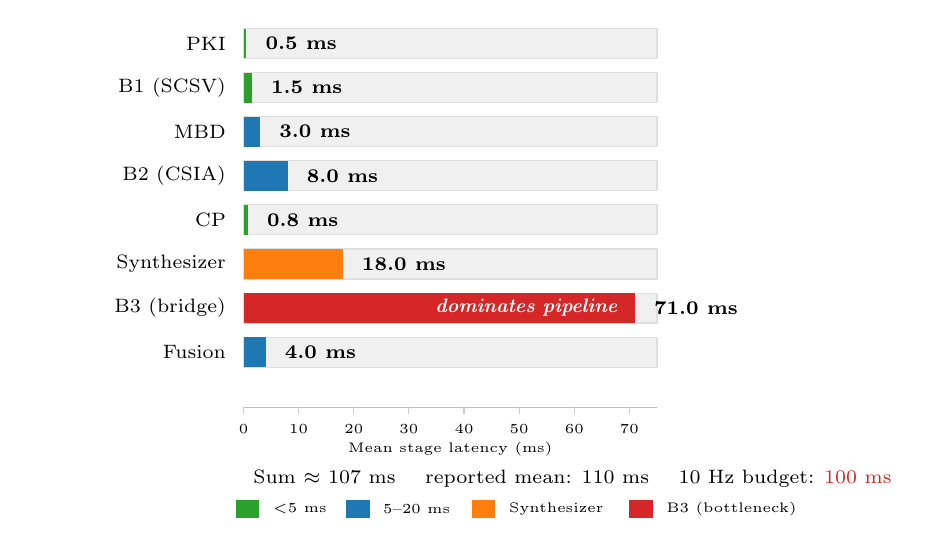
\begin{tikzpicture}[
  every node/.style={font=\scriptsize\sffamily},
]

\definecolor{headerblue}{RGB}{31,119,180}
\definecolor{barB3}{RGB}{214,39,40}
\definecolor{barSyn}{RGB}{255,127,14}
\definecolor{barMid}{RGB}{31,119,180}
\definecolor{barLow}{RGB}{44,160,44}
\definecolor{budget}{RGB}{214,39,40}

% ============================================================
% DATA
% layer name, latency (ms), color
% ============================================================
% Scale: \barscale cm per ms, max ~75 ms -> fits in ~5.2cm
\def\barscale{0.070}  % cm per ms
\def\barH{0.38}       % bar height cm
\def\gap{0.18}        % gap between bars
\def\labelW{2.4}      % label column width cm
\def\valoffset{0.12}  % gap after bar before value label

% Rows bottom to top (TikZ y increases upward, so row 0 is bottom)
% We'll go top to bottom: row 0 = PKI at top
% Latency values (ms):
%  0: PKI        0.5
%  1: B1 (SCSV)  1.5
%  2: MBD        3.0
%  3: B2 (CSIA)  8.0
%  4: CP         0.8
%  5: Synthesizer 18.0
%  6: B3 (bridge) 71.0
%  7: Fusion      4.0

\def\totalrows{8}

% Draw rows top to bottom
\foreach \r/\lbl/\val/\col in {
  0/PKI/0.5/barLow,
  1/B1 (SCSV)/1.5/barLow,
  2/MBD/3.0/barMid,
  3/B2 (CSIA)/8.0/barMid,
  4/CP/0.8/barLow,
  5/Synthesizer/18.0/barSyn,
  6/B3 (bridge)/71.0/barB3,
  7/Fusion/4.0/barMid}{
  \pgfmathsetmacro{\ypos}{-\r*(\barH+\gap)}
  % Row label
  \node[anchor=east, text width=\labelW cm, align=right,
        font=\scriptsize]
    at (\labelW, \ypos + 0.5*\barH) {\lbl};
  % Bar background (full scale)
  \fill[gray!12]
    (\labelW + 0.1, \ypos)
    rectangle +({75*\barscale}, \barH);
  \draw[gray!25, thin]
    (\labelW + 0.1, \ypos)
    rectangle +({75*\barscale}, \barH);
  % Actual bar
  \fill[\col]
    (\labelW + 0.1, \ypos)
    rectangle +({(\val)*\barscale}, \barH);
  % Value label
  \pgfmathsetmacro{\barend}{\labelW + 0.1 + (\val)*\barscale}
  \node[anchor=west, font=\scriptsize\bfseries]
    at (\barend + \valoffset, \ypos + 0.5*\barH)
    {\val\ ms};
}

% ============================================================
% X AXIS
% ============================================================
\pgfmathsetmacro{\axisy}{-\totalrows*(\barH+\gap)+0.05}
\draw[gray!50, thin]
  (\labelW + 0.1, \axisy) -- (\labelW + 0.1 + 75*\barscale, \axisy);

% X axis ticks
\foreach \v in {0,10,20,30,40,50,60,70}{
  \pgfmathsetmacro{\xpos}{\labelW + 0.1 + \v*\barscale}
  \draw[gray!40, thin] (\xpos, \axisy) -- (\xpos, \axisy - 0.08);
  \node[font=\tiny, text=black, anchor=north]
    at (\xpos, \axisy - 0.10) {\v};
}
\node[font=\tiny, text=black, anchor=north]
  at (\labelW + 0.1 + 37.5*\barscale, \axisy - 0.32)
  {Mean stage latency (ms)};

% ============================================================
% B3 "dominates pipeline" ANNOTATION
% [LAYOUT] Moved INSIDE the B3 bar (white text, anchor=east) to completely
%          eliminate any possibility of overlapping the Synthesizer row above it.
% Note: macro renamed to \bthreeypos to avoid clash with LaTeX \b accent.
\pgfmathsetmacro{\bthreeypos}{-6*(\barH+\gap)}
\node[
  font=\scriptsize\bfseries\itshape, text=white, align=right,
  anchor=east
] at (\labelW + 0.1 + 71*\barscale - 0.1, \bthreeypos + 0.5*\barH)
  {dominates pipeline};

% ============================================================
% TOTAL ANNOTATION
% ============================================================
\node[
  font=\scriptsize, text=black, align=left,
  anchor=west
] at (\labelW + 0.1, {-\totalrows*(\barH+\gap) - 0.85})
  {Sum $\approx$ 107 ms \quad reported mean: 110 ms \quad
   10 Hz budget: \textcolor{budget}{100 ms}};

% ============================================================
% LEGEND
% ============================================================
\pgfmathsetmacro{\legY}{-\totalrows*(\barH+\gap) - 1.35}

\fill[barLow]  (\labelW + 0.0, \legY)
  rectangle +(0.30, 0.22);
\node[font=\tiny, anchor=west]
  at (\labelW + 0.35, \legY + 0.11)
  {$<$5 ms};

\fill[barMid]  (\labelW + 1.4, \legY)
  rectangle +(0.30, 0.22);
\node[font=\tiny, anchor=west]
  at (\labelW + 1.75, \legY + 0.11)
  {5--20 ms};

\fill[barSyn]  (\labelW + 3.0, \legY)
  rectangle +(0.30, 0.22);
\node[font=\tiny, anchor=west]
  at (\labelW + 3.35, \legY + 0.11)
  {Synthesizer};

\fill[barB3]   (\labelW + 5.0, \legY)
  rectangle +(0.30, 0.22);
\node[font=\tiny, anchor=west]
  at (\labelW + 5.35, \legY + 0.11)
  {B3 (bottleneck)};

\end{tikzpicture}

%     \caption{Per-stage mean latency breakdown measured on the
%     120-scenario diagnostic harness. B3 (bridge + DeBERTa inference)
%     dominates at $\sim$71~ms. Total pipeline mean is 110~ms
%     (Section~VI-G); the 10~Hz CAM budget is 100~ms.}
%     \label{fig:perlayer_latency}
%   \end{figure}
% ============================================================

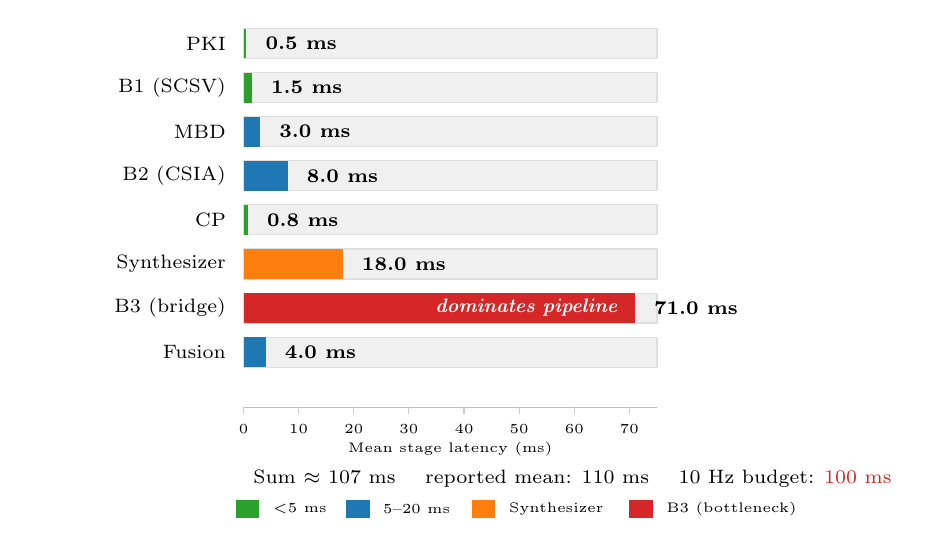
\begin{tikzpicture}[
  every node/.style={font=\scriptsize\sffamily},
]

\definecolor{headerblue}{RGB}{31,119,180}
\definecolor{barB3}{RGB}{214,39,40}
\definecolor{barSyn}{RGB}{255,127,14}
\definecolor{barMid}{RGB}{31,119,180}
\definecolor{barLow}{RGB}{44,160,44}
\definecolor{budget}{RGB}{214,39,40}

% ============================================================
% DATA
% layer name, latency (ms), color
% ============================================================
% Scale: \barscale cm per ms, max ~75 ms -> fits in ~5.2cm
\def\barscale{0.070}  % cm per ms
\def\barH{0.38}       % bar height cm
\def\gap{0.18}        % gap between bars
\def\labelW{2.4}      % label column width cm
\def\valoffset{0.12}  % gap after bar before value label

% Rows bottom to top (TikZ y increases upward, so row 0 is bottom)
% We'll go top to bottom: row 0 = PKI at top
% Latency values (ms):
%  0: PKI        0.5
%  1: B1 (SCSV)  1.5
%  2: MBD        3.0
%  3: B2 (CSIA)  8.0
%  4: CP         0.8
%  5: Synthesizer 18.0
%  6: B3 (bridge) 71.0
%  7: Fusion      4.0

\def\totalrows{8}

% Draw rows top to bottom
\foreach \r/\lbl/\val/\col in {
  0/PKI/0.5/barLow,
  1/B1 (SCSV)/1.5/barLow,
  2/MBD/3.0/barMid,
  3/B2 (CSIA)/8.0/barMid,
  4/CP/0.8/barLow,
  5/Synthesizer/18.0/barSyn,
  6/B3 (bridge)/71.0/barB3,
  7/Fusion/4.0/barMid}{
  \pgfmathsetmacro{\ypos}{-\r*(\barH+\gap)}
  % Row label
  \node[anchor=east, text width=\labelW cm, align=right,
        font=\scriptsize]
    at (\labelW, \ypos + 0.5*\barH) {\lbl};
  % Bar background (full scale)
  \fill[gray!12]
    (\labelW + 0.1, \ypos)
    rectangle +({75*\barscale}, \barH);
  \draw[gray!25, thin]
    (\labelW + 0.1, \ypos)
    rectangle +({75*\barscale}, \barH);
  % Actual bar
  \fill[\col]
    (\labelW + 0.1, \ypos)
    rectangle +({(\val)*\barscale}, \barH);
  % Value label
  \pgfmathsetmacro{\barend}{\labelW + 0.1 + (\val)*\barscale}
  \node[anchor=west, font=\scriptsize\bfseries]
    at (\barend + \valoffset, \ypos + 0.5*\barH)
    {\val\ ms};
}

% ============================================================
% X AXIS
% ============================================================
\pgfmathsetmacro{\axisy}{-\totalrows*(\barH+\gap)+0.05}
\draw[gray!50, thin]
  (\labelW + 0.1, \axisy) -- (\labelW + 0.1 + 75*\barscale, \axisy);

% X axis ticks
\foreach \v in {0,10,20,30,40,50,60,70}{
  \pgfmathsetmacro{\xpos}{\labelW + 0.1 + \v*\barscale}
  \draw[gray!40, thin] (\xpos, \axisy) -- (\xpos, \axisy - 0.08);
  \node[font=\tiny, text=black, anchor=north]
    at (\xpos, \axisy - 0.10) {\v};
}
\node[font=\tiny, text=black, anchor=north]
  at (\labelW + 0.1 + 37.5*\barscale, \axisy - 0.32)
  {Mean stage latency (ms)};

% ============================================================
% B3 "dominates pipeline" ANNOTATION
% [LAYOUT] Moved INSIDE the B3 bar (white text, anchor=east) to completely
%          eliminate any possibility of overlapping the Synthesizer row above it.
% Note: macro renamed to \bthreeypos to avoid clash with LaTeX \b accent.
\pgfmathsetmacro{\bthreeypos}{-6*(\barH+\gap)}
\node[
  font=\scriptsize\bfseries\itshape, text=white, align=right,
  anchor=east
] at (\labelW + 0.1 + 71*\barscale - 0.1, \bthreeypos + 0.5*\barH)
  {dominates pipeline};

% ============================================================
% TOTAL ANNOTATION
% ============================================================
\node[
  font=\scriptsize, text=black, align=left,
  anchor=west
] at (\labelW + 0.1, {-\totalrows*(\barH+\gap) - 0.85})
  {Sum $\approx$ 107 ms \quad reported mean: 110 ms \quad
   10 Hz budget: \textcolor{budget}{100 ms}};

% ============================================================
% LEGEND
% ============================================================
\pgfmathsetmacro{\legY}{-\totalrows*(\barH+\gap) - 1.35}

\fill[barLow]  (\labelW + 0.0, \legY)
  rectangle +(0.30, 0.22);
\node[font=\tiny, anchor=west]
  at (\labelW + 0.35, \legY + 0.11)
  {$<$5 ms};

\fill[barMid]  (\labelW + 1.4, \legY)
  rectangle +(0.30, 0.22);
\node[font=\tiny, anchor=west]
  at (\labelW + 1.75, \legY + 0.11)
  {5--20 ms};

\fill[barSyn]  (\labelW + 3.0, \legY)
  rectangle +(0.30, 0.22);
\node[font=\tiny, anchor=west]
  at (\labelW + 3.35, \legY + 0.11)
  {Synthesizer};

\fill[barB3]   (\labelW + 5.0, \legY)
  rectangle +(0.30, 0.22);
\node[font=\tiny, anchor=west]
  at (\labelW + 5.35, \legY + 0.11)
  {B3 (bottleneck)};

\end{tikzpicture}

%     \caption{Per-stage mean latency breakdown measured on the
%     120-scenario diagnostic harness. B3 (bridge + DeBERTa inference)
%     dominates at $\sim$71~ms. Total pipeline mean is 110~ms
%     (Section~VI-G); the 10~Hz CAM budget is 100~ms.}
%     \label{fig:perlayer_latency}
%   \end{figure}
% ============================================================

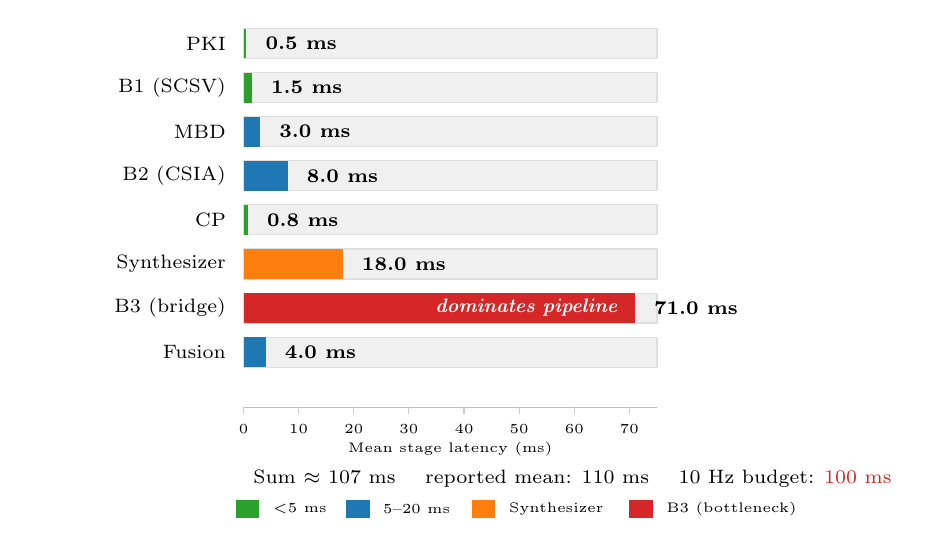
\begin{tikzpicture}[
  every node/.style={font=\scriptsize\sffamily},
]

\definecolor{headerblue}{RGB}{31,119,180}
\definecolor{barB3}{RGB}{214,39,40}
\definecolor{barSyn}{RGB}{255,127,14}
\definecolor{barMid}{RGB}{31,119,180}
\definecolor{barLow}{RGB}{44,160,44}
\definecolor{budget}{RGB}{214,39,40}

% ============================================================
% DATA
% layer name, latency (ms), color
% ============================================================
% Scale: \barscale cm per ms, max ~75 ms -> fits in ~5.2cm
\def\barscale{0.070}  % cm per ms
\def\barH{0.38}       % bar height cm
\def\gap{0.18}        % gap between bars
\def\labelW{2.4}      % label column width cm
\def\valoffset{0.12}  % gap after bar before value label

% Rows bottom to top (TikZ y increases upward, so row 0 is bottom)
% We'll go top to bottom: row 0 = PKI at top
% Latency values (ms):
%  0: PKI        0.5
%  1: B1 (SCSV)  1.5
%  2: MBD        3.0
%  3: B2 (CSIA)  8.0
%  4: CP         0.8
%  5: Synthesizer 18.0
%  6: B3 (bridge) 71.0
%  7: Fusion      4.0

\def\totalrows{8}

% Draw rows top to bottom
\foreach \r/\lbl/\val/\col in {
  0/PKI/0.5/barLow,
  1/B1 (SCSV)/1.5/barLow,
  2/MBD/3.0/barMid,
  3/B2 (CSIA)/8.0/barMid,
  4/CP/0.8/barLow,
  5/Synthesizer/18.0/barSyn,
  6/B3 (bridge)/71.0/barB3,
  7/Fusion/4.0/barMid}{
  \pgfmathsetmacro{\ypos}{-\r*(\barH+\gap)}
  % Row label
  \node[anchor=east, text width=\labelW cm, align=right,
        font=\scriptsize]
    at (\labelW, \ypos + 0.5*\barH) {\lbl};
  % Bar background (full scale)
  \fill[gray!12]
    (\labelW + 0.1, \ypos)
    rectangle +({75*\barscale}, \barH);
  \draw[gray!25, thin]
    (\labelW + 0.1, \ypos)
    rectangle +({75*\barscale}, \barH);
  % Actual bar
  \fill[\col]
    (\labelW + 0.1, \ypos)
    rectangle +({(\val)*\barscale}, \barH);
  % Value label
  \pgfmathsetmacro{\barend}{\labelW + 0.1 + (\val)*\barscale}
  \node[anchor=west, font=\scriptsize\bfseries]
    at (\barend + \valoffset, \ypos + 0.5*\barH)
    {\val\ ms};
}

% ============================================================
% X AXIS
% ============================================================
\pgfmathsetmacro{\axisy}{-\totalrows*(\barH+\gap)+0.05}
\draw[gray!50, thin]
  (\labelW + 0.1, \axisy) -- (\labelW + 0.1 + 75*\barscale, \axisy);

% X axis ticks
\foreach \v in {0,10,20,30,40,50,60,70}{
  \pgfmathsetmacro{\xpos}{\labelW + 0.1 + \v*\barscale}
  \draw[gray!40, thin] (\xpos, \axisy) -- (\xpos, \axisy - 0.08);
  \node[font=\tiny, text=black, anchor=north]
    at (\xpos, \axisy - 0.10) {\v};
}
\node[font=\tiny, text=black, anchor=north]
  at (\labelW + 0.1 + 37.5*\barscale, \axisy - 0.32)
  {Mean stage latency (ms)};

% ============================================================
% B3 "dominates pipeline" ANNOTATION
% [LAYOUT] Moved INSIDE the B3 bar (white text, anchor=east) to completely
%          eliminate any possibility of overlapping the Synthesizer row above it.
% Note: macro renamed to \bthreeypos to avoid clash with LaTeX \b accent.
\pgfmathsetmacro{\bthreeypos}{-6*(\barH+\gap)}
\node[
  font=\scriptsize\bfseries\itshape, text=white, align=right,
  anchor=east
] at (\labelW + 0.1 + 71*\barscale - 0.1, \bthreeypos + 0.5*\barH)
  {dominates pipeline};

% ============================================================
% TOTAL ANNOTATION
% ============================================================
\node[
  font=\scriptsize, text=black, align=left,
  anchor=west
] at (\labelW + 0.1, {-\totalrows*(\barH+\gap) - 0.85})
  {Sum $\approx$ 107 ms \quad reported mean: 110 ms \quad
   10 Hz budget: \textcolor{budget}{100 ms}};

% ============================================================
% LEGEND
% ============================================================
\pgfmathsetmacro{\legY}{-\totalrows*(\barH+\gap) - 1.35}

\fill[barLow]  (\labelW + 0.0, \legY)
  rectangle +(0.30, 0.22);
\node[font=\tiny, anchor=west]
  at (\labelW + 0.35, \legY + 0.11)
  {$<$5 ms};

\fill[barMid]  (\labelW + 1.4, \legY)
  rectangle +(0.30, 0.22);
\node[font=\tiny, anchor=west]
  at (\labelW + 1.75, \legY + 0.11)
  {5--20 ms};

\fill[barSyn]  (\labelW + 3.0, \legY)
  rectangle +(0.30, 0.22);
\node[font=\tiny, anchor=west]
  at (\labelW + 3.35, \legY + 0.11)
  {Synthesizer};

\fill[barB3]   (\labelW + 5.0, \legY)
  rectangle +(0.30, 0.22);
\node[font=\tiny, anchor=west]
  at (\labelW + 5.35, \legY + 0.11)
  {B3 (bottleneck)};

\end{tikzpicture}

%     \caption{Per-stage mean latency breakdown measured on the
%     120-scenario diagnostic harness. B3 (bridge + DeBERTa inference)
%     dominates at $\sim$71~ms. Total pipeline mean is 110~ms
%     (Section~VI-G); the 10~Hz CAM budget is 100~ms.}
%     \label{fig:perlayer_latency}
%   \end{figure}
% ============================================================

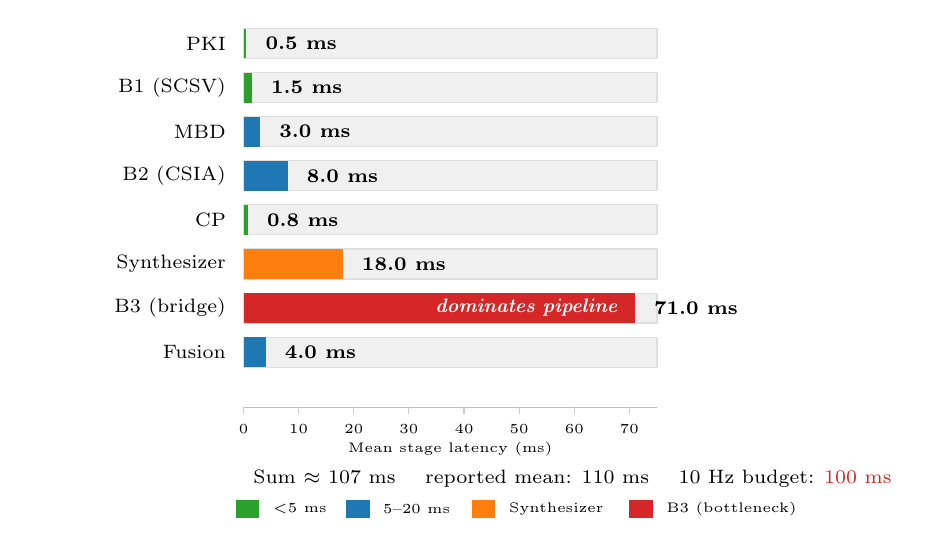
\begin{tikzpicture}[
  every node/.style={font=\scriptsize\sffamily},
]

\definecolor{headerblue}{RGB}{31,119,180}
\definecolor{barB3}{RGB}{214,39,40}
\definecolor{barSyn}{RGB}{255,127,14}
\definecolor{barMid}{RGB}{31,119,180}
\definecolor{barLow}{RGB}{44,160,44}
\definecolor{budget}{RGB}{214,39,40}

% ============================================================
% DATA
% layer name, latency (ms), color
% ============================================================
% Scale: \barscale cm per ms, max ~75 ms -> fits in ~5.2cm
\def\barscale{0.070}  % cm per ms
\def\barH{0.38}       % bar height cm
\def\gap{0.18}        % gap between bars
\def\labelW{2.4}      % label column width cm
\def\valoffset{0.12}  % gap after bar before value label

% Rows bottom to top (TikZ y increases upward, so row 0 is bottom)
% We'll go top to bottom: row 0 = PKI at top
% Latency values (ms):
%  0: PKI        0.5
%  1: B1 (SCSV)  1.5
%  2: MBD        3.0
%  3: B2 (CSIA)  8.0
%  4: CP         0.8
%  5: Synthesizer 18.0
%  6: B3 (bridge) 71.0
%  7: Fusion      4.0

\def\totalrows{8}

% Draw rows top to bottom
\foreach \r/\lbl/\val/\col in {
  0/PKI/0.5/barLow,
  1/B1 (SCSV)/1.5/barLow,
  2/MBD/3.0/barMid,
  3/B2 (CSIA)/8.0/barMid,
  4/CP/0.8/barLow,
  5/Synthesizer/18.0/barSyn,
  6/B3 (bridge)/71.0/barB3,
  7/Fusion/4.0/barMid}{
  \pgfmathsetmacro{\ypos}{-\r*(\barH+\gap)}
  % Row label
  \node[anchor=east, text width=\labelW cm, align=right,
        font=\scriptsize]
    at (\labelW, \ypos + 0.5*\barH) {\lbl};
  % Bar background (full scale)
  \fill[gray!12]
    (\labelW + 0.1, \ypos)
    rectangle +({75*\barscale}, \barH);
  \draw[gray!25, thin]
    (\labelW + 0.1, \ypos)
    rectangle +({75*\barscale}, \barH);
  % Actual bar
  \fill[\col]
    (\labelW + 0.1, \ypos)
    rectangle +({(\val)*\barscale}, \barH);
  % Value label
  \pgfmathsetmacro{\barend}{\labelW + 0.1 + (\val)*\barscale}
  \node[anchor=west, font=\scriptsize\bfseries]
    at (\barend + \valoffset, \ypos + 0.5*\barH)
    {\val\ ms};
}

% ============================================================
% X AXIS
% ============================================================
\pgfmathsetmacro{\axisy}{-\totalrows*(\barH+\gap)+0.05}
\draw[gray!50, thin]
  (\labelW + 0.1, \axisy) -- (\labelW + 0.1 + 75*\barscale, \axisy);

% X axis ticks
\foreach \v in {0,10,20,30,40,50,60,70}{
  \pgfmathsetmacro{\xpos}{\labelW + 0.1 + \v*\barscale}
  \draw[gray!40, thin] (\xpos, \axisy) -- (\xpos, \axisy - 0.08);
  \node[font=\tiny, text=black, anchor=north]
    at (\xpos, \axisy - 0.10) {\v};
}
\node[font=\tiny, text=black, anchor=north]
  at (\labelW + 0.1 + 37.5*\barscale, \axisy - 0.32)
  {Mean stage latency (ms)};

% ============================================================
% B3 "dominates pipeline" ANNOTATION
% [LAYOUT] Moved INSIDE the B3 bar (white text, anchor=east) to completely
%          eliminate any possibility of overlapping the Synthesizer row above it.
% Note: macro renamed to \bthreeypos to avoid clash with LaTeX \b accent.
\pgfmathsetmacro{\bthreeypos}{-6*(\barH+\gap)}
\node[
  font=\scriptsize\bfseries\itshape, text=white, align=right,
  anchor=east
] at (\labelW + 0.1 + 71*\barscale - 0.1, \bthreeypos + 0.5*\barH)
  {dominates pipeline};

% ============================================================
% TOTAL ANNOTATION
% ============================================================
\node[
  font=\scriptsize, text=black, align=left,
  anchor=west
] at (\labelW + 0.1, {-\totalrows*(\barH+\gap) - 0.85})
  {Sum $\approx$ 107 ms \quad reported mean: 110 ms \quad
   10 Hz budget: \textcolor{budget}{100 ms}};

% ============================================================
% LEGEND
% ============================================================
\pgfmathsetmacro{\legY}{-\totalrows*(\barH+\gap) - 1.35}

\fill[barLow]  (\labelW + 0.0, \legY)
  rectangle +(0.30, 0.22);
\node[font=\tiny, anchor=west]
  at (\labelW + 0.35, \legY + 0.11)
  {$<$5 ms};

\fill[barMid]  (\labelW + 1.4, \legY)
  rectangle +(0.30, 0.22);
\node[font=\tiny, anchor=west]
  at (\labelW + 1.75, \legY + 0.11)
  {5--20 ms};

\fill[barSyn]  (\labelW + 3.0, \legY)
  rectangle +(0.30, 0.22);
\node[font=\tiny, anchor=west]
  at (\labelW + 3.35, \legY + 0.11)
  {Synthesizer};

\fill[barB3]   (\labelW + 5.0, \legY)
  rectangle +(0.30, 0.22);
\node[font=\tiny, anchor=west]
  at (\labelW + 5.35, \legY + 0.11)
  {B3 (bottleneck)};

\end{tikzpicture}
